
\begin{lemma}{Mitternachtsformel}
    $x=\frac{-b\pm\sqrt{b^2-4ac}}{2a}$
\end{lemma}

\begin{formula}{Polynomdivision} \emph{!} Vorzeichen von Nullstellen umdrehen\\
    $\frac{P(x)}{q(x)} = S(x) + \frac{r(x)}{q(x)}$ \qquad $P,q,S,r$ Polynome
$$
\begin{array}{cc}
\left(x^3-2 x^2-5 x-6\right):(x-1)=x^2-x-6 & \mid x^3: x=x^2 \\
-\left(x^3-x^2\right) & \mid-x^2: x=-x \\
-x^2-5 x & \\
-\left(x^2-x\right) & \mid-6 x: x=-6 \\
\hline-(-6 x+6) &
\end{array}
$$

Eine Polynomfunktion vom Grad $n$ hat höchstens $n$ reelle Nullstellen.
$$
f(x)=a_n \cdot\left(x-x_1\right) \cdot\left(x-x_2\right) \cdot \ldots \cdot\left(x-x_n\right)
$$
\end{formula}

\begin{definition}{Kardinalität}
    \begin{itemize}
        \item X, Y \emph{gleichmächtig}, falls es eine \underline{Bijektion} $f: X \to Y$ gibt.
        \item X \emph{endlich}, falls entweder $X = \emptyset$ ($\card X = 0$) oder $\exists n \in \N$, sodass $X$ und $\{1,2,\ldots,n\}$ ($\card X = n$) gleichmächtig sind.
        \item X \emph{abzählbar}, falls sie endlich oder gleichmächtig wie $\N$ ist.
    \end{itemize}
\end{definition}
\begin{definition}{Beschränktheit}
    $A \subseteq \R$ eine Teilmenge.
    \begin{itemize}
        \item $c \in \R$ ist eine \emph{obere Schranke} von A falls $\forall a \in A: a\leq c$ ($A$ \textit{nach oben beschränkt}).
        \item $c \in \R$ ist eine \emph{untere Schranke} von A falls $\forall a \in A: a \geq c$ ($A$ \textit{nach unten beschränkt}).
        \item $A$ heisst \textit{beschränkt}, wenn nach oben und unten beschränkt.
        \item \emph{Maximum} von $A$ falls $m \in A$ und $m$ obere Schranke.
        \item \emph{Minimum} von $A$ falls $m \in A$ und $m$ untere Schranke.
    \end{itemize}
\end{definition}


\begin{definition}{Intervalle}
    Ein \emph{abgeschlossenes Intervall} ist eine Teilmenge $I \subseteq \R$ der Form
    \begin{itemize}
        \item Abgeschlossen:
            $[a, b]=\{x \in \mathbb{R} \mid a \leq x \leq b\}$
        \item Offen:
            $(a, b)=\{x \in \mathbb{R} \mid a<x<b\}$
        \item Halboffen:
            $[a, b)=\{x \in \mathbb{R} \mid a \leq x<b\}$
        \item Unendlich:
            $[a, \infty)=\{x \in \mathbb{R} \mid a \leq x\}$
    \end{itemize}
\end{definition}

\begin{definition}{Supremum und Infimum}
    $A \subseteq \R, ~A\neq \emptyset$
    \begin{enumerateroman}
        \item $A$ nach oben beschränkt. Dann gibt es eine kleinste obere Schranke von $A$: $c \coloneqq \sup A$. Das \emph{Supremum} von $A$.
        \item $A$ nach unten beschränkt. Dann gibt es eine kleinste untere Schranke von $A$: $c \coloneqq \inf A$. Das \emph{Infimum} von $A$.
    \end{enumerateroman}
    \tcblower 
    Vereinfacht formuliert: Für ein abgeschlossenes, halboffenes oder offenes Intervall $[a,b], [a,b), (a,b]$ oder $(a,b)$ gilt $inf = a$, $sup = b$ (solange $a, b \neq \infty$)
\end{definition}

\begin{definition}{Monotonie}
    \begin{enumerate}
        \item $\sequence$ \emph{monoton wachsend} falls: \null\hfill $a_n \leq a_{n + 1} \quad \forall n \geq 1$.
    	\item $\sequence$ \emph{monoton fallend} falls: \null\hfill $a_n \geq a_{n+1} \quad \forall n \geq 1$.
    \end{enumerate}
\end{definition}

\begin{KR}{Monotonie zeigen}
    \begin{itemize}
  \item $a_{n+1}-a_{n} \geq 0 \Rightarrow$ monoton wachsend (bzw. umgekehrt fallend)
  \item $\frac{a_{n+1}}{a_{n}} \geq 1$ und $a_{n} \geq 0$ dann monoton wachsend
\end{itemize}
\end{KR}

\raggedcolumns
\columnbreak

\subsubsection{Trigonometrische Funktionen}

\begin{iequation}[align*]
	\tikz[remember picture] \coordinate(sinanchor) at (0,0); \sin x &= \sum_{n=0}^{\infty} \frac{(-1)^n x^{2n + 1}}{(2n+1)!} = x - \frac{x^3}{3!} + \frac{x^5}{5!}\ldots ~ \text{stetig}\\
	\tikz[remember picture] \coordinate(cosanchor) at (0,0); \cos x &= \sum_{n=0}^{\infty} \frac{(-1)^n x^{2n}}{(2n)!} = 1 - \frac{x^2}{2!} + \frac{x^4}{4!}\ldots \hspace{3.8mm} \text{stetig}\\
	\tan x &= \frac{\sin x}{\cos x} \hspace{10mm} \cot x = \frac{\cos x}{\sin x} \tikz[remember picture] \coordinate(trigfunkanchor) at (0,0);
\end{iequation}
\begin{tikzpicture}[remember picture, overlay]
	\node[overlaynote, text width = 28mm, anchor = west] at ($(trigfunkanchor) + (0.5,0.25)$) {$\pi$: kleinste strikt positive Nullstelle von $\sin$.};
	\node[overlaynote, rotate = 90] at ($(trigfunkanchor) + (3,2)$) {$\cos(x) = \sin \left(x + \frac{\pi}{2}\right)$};
	\node[overlaynote, rotate = 20, above left = 3mm and 2mm of sinanchor] (sinnote) {ungerade};
	\draw[overlayarrow] (sinnote) to[bend right] (sinanchor);
	\node[overlaynote, rotate = 20, above left = 3mm and 2mm of cosanchor] (cosnote) {gerade};
	\draw[overlayarrow] (cosnote) to[bend right] (cosanchor);
\end{tikzpicture}

\begin{center}
    \renewcommand{\arraystretch}{1.3} %Zeilenabstand verändern
    \setlength{\tabcolsep}{4pt}
    \begin{tabular}{|c|c|c|c|c|c|c|c|c|c|}
        \hline
        Grad            & $0^\circ$ & $30^\circ$           & $45^\circ$           & $60^\circ$           & $90^\circ$      & $120^\circ$          & $135^\circ$           & $150^\circ$           & $180^\circ$ \\
        \hline
        $\varphi$       & $0$       & $\frac{\pi}{6}$      & $\frac{\pi}{4}$      & $\frac{\pi}{3}$      & $\frac{\pi}{2}$ & $\frac{2\pi}{3}$     & $\frac{3\pi}{4}$      & $\frac{5\pi}{6}$      & $\pi$       \\
        \hline
        $\sin(\varphi)$ & $0$       & $\frac{1}{2}$        & $\frac{\sqrt{2}}{2}$ & $\frac{\sqrt{3}}{2}$ & $1$             & $\frac{\sqrt{3}}{2}$ & $\frac{\sqrt{2}}{2}$  & $\frac{1}{2}$         & $0$         \\
        \hline
        $\cos(\varphi)$ & $1$       & $\frac{\sqrt{3}}{2}$ & $\frac{\sqrt{2}}{2}$ & $\frac{1}{2}$        & $0$             & $-\frac{1}{2}$       & $-\frac{\sqrt{2}}{2}$ & $-\frac{\sqrt{3}}{2}$ & $-1$        \\
        \hline
        $\tan(\varphi)$ & $0$       & $\frac{\sqrt{3}}{3}$ & $1$                  & $\sqrt{3}$           & $\pm \infty$    & -$\sqrt{3}$          & $-1$                  & $-\frac{\sqrt{3}}{3}$ & $0$         \\
        \hline
    \end{tabular}
\end{center}





\begin{theorem}{Eigenschaften sin/cos}
    \begin{enumerate}
        \item $\exp ix = \cos(x) + i \sin(x) \quad \forall x \in \mathbb{C}$
        \item $\cos x = \cos(-x) ~\text{und}~ \sin(-x) = -\sin x \quad\forall x \in \mathbb{C}$
        \item $\sin(x + y) = \sin(x)\cos(y) + \cos(x)\sin(y)$
        \item $\cos(x + y) = \cos(x)\cos(y) - \sin(x)\sin(y)$
        \item $\cos^2(x) + \sin^2(x) = 1 \quad \forall x \in \mathbb{C}$ 
        \item $\sin x = \frac{e^{iz} - e^{-iz}}{2i}, \quad \cos x = \frac{e^{iz} + e^{-iz}}{2}$
    \end{enumerate} 
 \end{theorem}
 
 \begin{corollary}{Winkelverdopplung}\\
         $\sin(2x) = 2 \sin(x)\cos(x)$ \hspace{4mm} $\cos(2x) = \cos^2(x) - \sin^2(x)$
 \end{corollary}
 \begin{corollary}{Potenz der Winkelfunktion}\\
    $$\sin^2(x) = \frac{1 - \cos(2x)}{2} \quad \cos^2(x) = \frac{1 + \cos(2x)}{2}$$
     %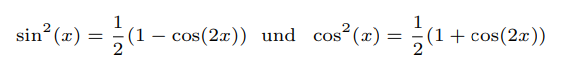
\includegraphics[scale=0.5]{Analysis1/zsf/Images/Basics/potenz_winkelfunktion.png}
 \end{corollary}
 \begin{corollary}{Eigenschaften mit $\pi$}
     \begin{enumerate}[itemsep= 2pt]
         \item $e^{i\pi} = -1, \quad e^{2i\pi} = 1$
         \item $\sin\left(x + \frac{\pi}{2}\right) = \cos(x), \quad \cos\left(x + \frac{\pi}{2}\right) = -\sin(x)$
         \item $\sin(x+\pi) = -\sin (x), \quad \sin(x + 2\pi) = \sin(x)$
         \item $\cos(x+\pi) = -\cos (x), \quad \cos(x + 2\pi) = \cos(x)$
     \end{enumerate}
 \end{corollary}

 \begin{corollary}{Nullstellen von trigonometrischen Funktionen}
    \begin{enumerate}
         \item $\text{Nullstellen Sinus} = \{k\cdot \pi : k\in \mathbb{Z}\}$\\
        $\sin(x) > 0 \quad \forall x \in ]2k\pi, ~(2k+1)\pi[, ~ k\in \mathbb{Z}$\\[2pt]
        $\sin(x) < 0 \quad \forall x \in ](2k + 1)\pi, ~(2k+2)\pi[, ~ k\in \mathbb{Z}$
        \item $\text{Nullstellen Cosinus} = \left\{\frac{\pi}{2}+k\cdot \pi : k\in \mathbb{Z}\right\}$\\
        $\cos(x) > 0:\forall x \in \left]-\frac{\pi}{2} +2k\pi, ~-\frac{\pi}{2} +(2k+1)\pi\right[, ~ k\in \mathbb{Z}$\\[2pt]
        $\cos(x) < 0:\forall x \in \left]-\frac{\pi}{2} + (2k + 1)\pi, ~-\frac{\pi}{2} +(2k+2)\pi\right[, ~ k\in \mathbb{Z}$
    \end{enumerate}
\end{corollary}
\noindent Für $\tan(x)$ gilt $x \notin \frac{\pi}{2} + \pi \cdot \Z$ \qquad Für $\cot(x)$ gilt $x \notin \pi \Z$
 

\raggedcolumns
\columnbreak

\subsubsection{Relle Exponentialfunktion}
\begin{center}
    \hfill
    \begin{minipage}{0.3\linewidth}
        \begin{iequation}
            \exp (z) \coloneqq \sum_{n=0}^\infty \frac{z^n}{n!}
        \end{iequation}
    \end{minipage}
    \hfill
    \begin{minipage}{0.6\linewidth}
        \begin{theorem}{Eigenschaften}
            $\exp : \R \to ]0, + \infty[$ ist streng monoton wachsend, stetig und surjektiv.
        \end{theorem}       
    \end{minipage}
    \hfill
\end{center}

%\begin{center}
    \begin{minipage}{0.5\linewidth}
        \begin{iequation}[align*]
            \exp(-x)\exp(x) &= 1\\
	    \text{\textbf{\textsf{}}} \quad\exp(x) &> 0 \qquad\forall x \in \R \tikz[remember picture, overlay]
	    \coordinate(expineq) at (0,0);\\
            \exp(x) &> 1 \qquad\forall x > 0\\
            \exp(a+b) &= \exp(a) \cdot \exp(b)\\ 
            \exp(a-b) &= \exp(a) \div \exp(b)
        \end{iequation}
\begin{tikzpicture}[overlay, remember picture]
	\node[overlaynote, above right = 8mm and 0mm of expineq] (expineqnote) {Aber nicht: $\exp(z) > 0 \quad \forall z \in \C$};
\end{tikzpicture}
    \end{minipage}
    \hfill
    \begin{minipage}{0.48\linewidth}
        \begin{corollary}
            \\$\exp(z) > \exp(y) \quad \forall z > y$
        \end{corollary}
        \begin{corollary}
            \\${\exp (x) \geq 1 + x \quad \forall x \in \R}$
        \end{corollary}    
        \begin{corollary}
            \\$e^{\alpha x} = \sum_{n=0}^\infty \frac{\alpha^n x^n}{n!}$
        \end{corollary}
    \end{minipage}
%\end{center}
$\exp(z) = \exp(y + (z-y)) = \exp(y) \exp(z-y)\\
            \exp(x) = \lim_{n\to \infty}(1 + \frac{x}{n})^n$\\
 \begin{minipage}{0.6\linewidth}
        \begin{align*}
            \exp(\ln a + \ln b) &= \exp(\ln a) \cdot \exp (\ln b)\\
            \exp(\ln a)\exp(\ln b) &= ab = \exp(\ln ab)\\
            \exp(\ln a + \ln b) &= \exp(\ln ab)\\
            \ln a + \ln b &= \ln (ab)
        \end{align*}
    \end{minipage}
    \hfill
    \begin{minipage}{0.35\linewidth}
        \begin{iequation}
            x^a \coloneqq \exp(a \ln x)
        \end{iequation}
    \end{minipage}

    \subsubsection*{Logarithmen}
\begin{corollary}{Rechnen mit Logarithmen}
    \begin{enumerate}
        \item Für $a > 0$ ist $]0, \infty[ \to ]0 + \infty[$ \quad $x \mapsto x^a$ eine stetige, streng monoton wachsende Bijektion.
        \item Für $a < 0$ ist $]0, \infty[ \to ]0 + \infty[$ \quad $x \mapsto x^a$ eine stetige, streng monoton fallende Bijektion.
        \item $\ln (a \cdot b) = \ln a + \ln b \quad \forall a,b \in ]0 +  \infty[$
        \item $\ln (a \div b) = \ln a - \ln b \quad \forall a,b \in ]0 +  \infty[$
        \item ${\ln \left(x^a\right) = a \ln (x) \quad \forall a \in \R, \forall x > 0}$
        \item ${x^a \cdot x^b = x^{a+b} \quad a,b \in \R, \forall x > 0}$
        \item ${\left(x^a\right)^b = x^{a \cdot b} \quad \forall a,b \in \R, \forall x > 0}$
    \end{enumerate}
    Im Allgemeinen gilt: $log_b (a) = \frac{ln(a)}{ln(b)}$
\end{corollary}

\begin{formula}{ln(1 + x)}
       $ = \sum_{n=1}^\infty \frac{(-1)^{n-1}x^n}{n} \quad \text{für} \quad |x| < 1$
\end{formula}

\subsubsection{Werte von log}
\begin{equation*}
	\begin{array}{lccccccc}
		& 0 & 1 & 2 & e & 3 & 5 & 10\\
		\ln & - \infty & 0 & 0.693 & 1 & 1.09 & 1.609 & 2.303\\
		\log_2 & - \infty & 0 & 1 & 1.443 & 1.585 & 2.321 & 3.321\\
		\log_{10} & - \infty & 0 & 0.301 & 0.434 & 0.477 & 0.699 & 1
	\end{array}
\end{equation*}

\begin{center}
    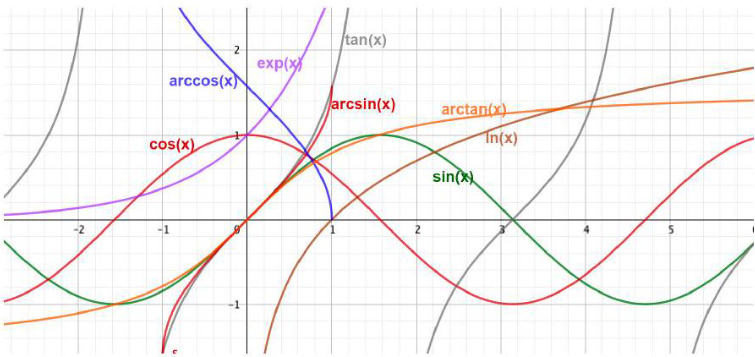
\includegraphics[width=0.8\linewidth]{trigonometrische_funktionen.png}
\end{center}









